\section{これについて} \label{sec:introduction}

\subsubsection{状況:}

当初開発を始めたサイクルにおいて、途中で何をすべきかわからなくなったため、新しいサイクルとして仕切り直すこととした。 \\
これまでの開発を第1サイクルとし、今後の開発を第2, 第3, ...サイクルとする。 \\
なお第2サイクルに入る前に、第1サイクルの事後分析を行い、プロジェクトとしての計画を立てるため、第1サイクルの戦略をする。 \\

現在までの状況と、今後どう進めるかは次のイメージ \\

\begin{figure}[H]
  \centering
  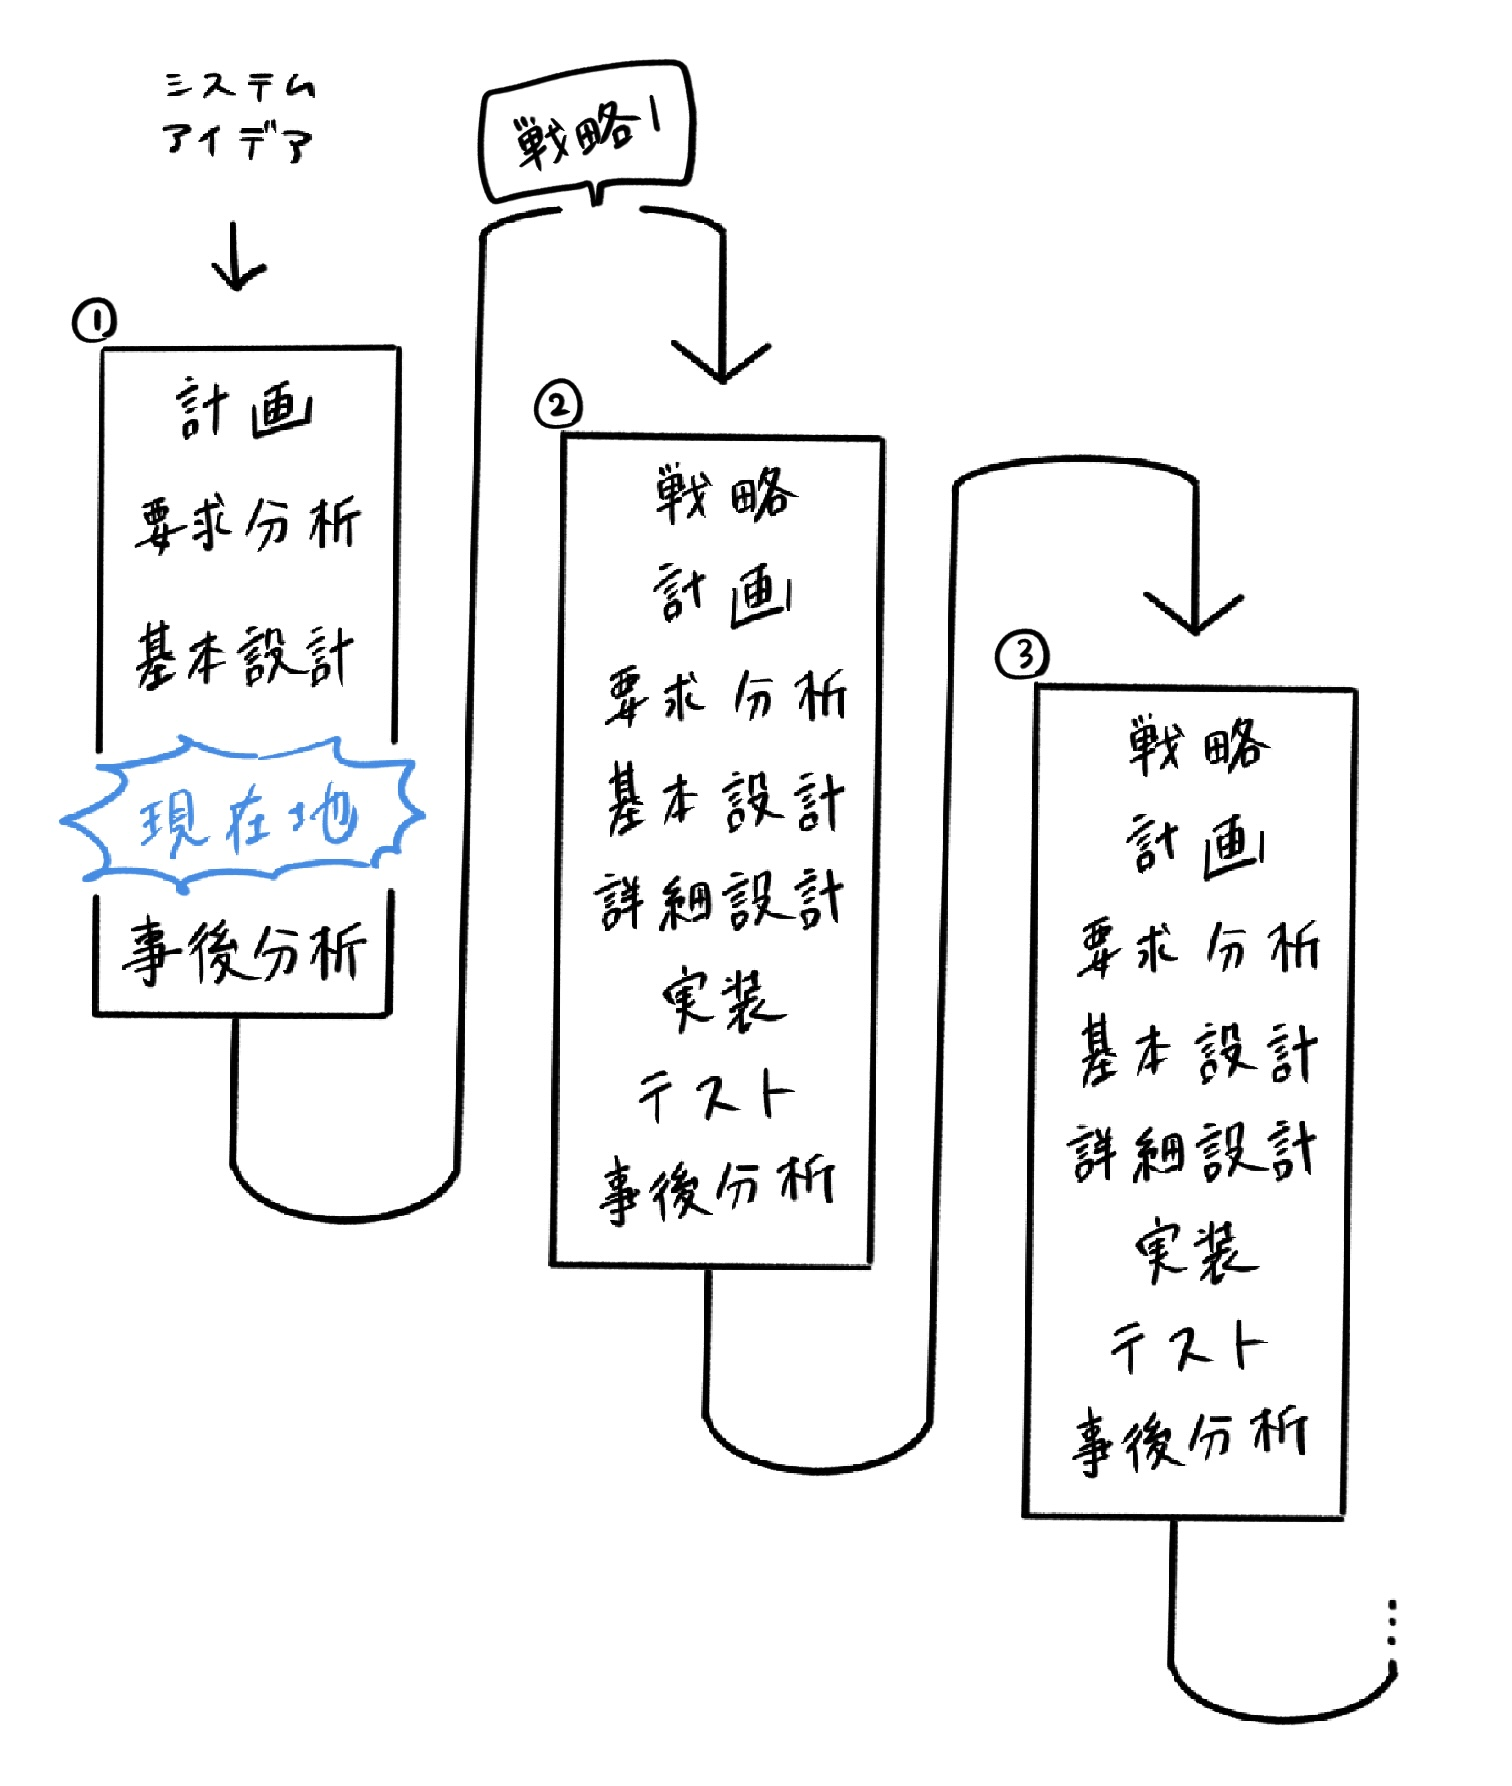
\includegraphics[width=80mm]{sections/cycle.jpg}
  \caption{サイクルの進め方}
  \label{fig:output}
\end{figure}

そこで、議事録という面を含むが、この文書で記述するのは次のとおり.

\begin{itemize}
  \item これまでの事後分析
  \item 本来すべきだった第1サイクルの戦略
  \begin{itemize}
    \item 概念設計
    \item 最終的にシステムが完成するまでの時間見積もり
    \item サイクル分割
  \end{itemize}
  \item これからのサイクルの進め方
\end{itemize}

